\documentclass[14pt,compress,english,utf8,t]{beamer}

\usepackage{etex}

\usepackage[english]{babel}

\usepackage{tikz}
\usepackage{booktabs}
\usepackage{ragged2e}
\usepackage{mathtools}
\usepackage{wasysym}

\usepackage{minted}
\usemintedstyle{tango}


\usetikzlibrary{calc,shapes.callouts,shapes.arrows}
\definecolor{darkred}{RGB}{220,0,0}
\newcommand{\hcancel}[5]{%
    \tikz[baseline=(tocancel.base)]{
        \node[inner sep=0pt,outer sep=0pt] (tocancel) {#1};
        \draw[darkred, line width=1mm] ($(tocancel.south west)+(#2,#3)$) -- ($(tocancel.north east)+(#4,#5)$);
    }%
}%

\usepackage[protrusion=true,expansion=true]{microtype}

\title[10 modern programming concepts]{10 modern programming concepts \\ which
your favourite programming language is missing\footnote{unless your favorite
language is \ldots}}
\author[Curry Club Augsburg]{
\includegraphics[scale=0.6]{logo-heller-hintergrund}}
\institute{32th Chaos Communication Congress}
\date{December 29th, 2015}

\usetheme{Warsaw}
\usecolortheme{seahorse}
\definecolor{mypurple}{RGB}{150,0,255}
\setbeamercolor{structure}{fg=mypurple}
\usefonttheme{serif}
\usepackage[T1]{fontenc}
\usepackage{libertine}
\useinnertheme{rectangles}
\setbeamercovered{invisible}

\setbeamertemplate{title page}[default][colsep=-1bp,rounded=false,shadow=false]
\setbeamertemplate{frametitle}[default][colsep=-2bp,rounded=false,shadow=false,center]

\setbeamertemplate{navigation symbols}{}
\setbeamertemplate{headline}{}

\newcommand*\oldmacro{}%
\let\oldmacro\insertshorttitle%
\renewcommand*\insertshorttitle{%
  \oldmacro\hfill\insertframenumber\,/\,\inserttotalframenumber\hfill}

\newcommand{\defeq}{\vcentcolon=}

\newcommand{\hil}[1]{{\usebeamercolor[fg]{item}{\textbf{#1}}}}

\newcommand{\atpos}[1]{%
  \begin{tikzpicture}[remember picture, overlay]%
    \node[anchor=south east] at (current page.south east) {#1};
  \end{tikzpicture}%
}

\newcommand{\centeredpar}[2]{%
  \begin{center}
    \colorbox{white}{\parbox{#1\textwidth}{%
      #2%
    }}%
  \end{center}%
}

\newcommand{\icfrac}[4]{#1 + \dfrac{1}{#2 + \dfrac{1}{#3 + \dfrac{1}{#4 + \ddots}}}}
\newcommand{\icfracc}[3]{\dfrac{1}{#1 + \dfrac{1}{#2 + \dfrac{1}{#3 + \ddots}}}}
\newcommand{\icfraccc}[2]{\dfrac{1}{#1 + \dfrac{1}{#2 + \ddots}}}
\newcommand{\icfracccc}[5]{#1 + \dfrac{1}{#2 + \dfrac{1}{#3 + \dfrac{1}{#4 + \dfrac{1}{#5 + \ddots}}}}}

% Gonzalo Medina, http://tex.stackexchange.com/a/228198
\makeatletter
\def\Mdescription#1{%
  \advance\beamer@descdefault by \labelsep%
  \list
  {}
  {\labelwidth\beamer@descdefault%
  \leftmargin\beamer@descdefault%
  \let\makelabel\beamer@descriptionitem
  \settowidth\labelwidth{\beamer@descriptionitem{#1}}%
  \setlength\leftmargin{\labelwidth}% 
  \addtolength\leftmargin{\labelsep}%
  }%
  \beamer@cramped%
  \raggedright
  \beamer@firstlineitemizeunskip%
}
\def\endMdescription{\ifhmode\unskip\fi\endlist}
\long\def\beamer@descriptionitem#1{%
  \def\insertdescriptionitem{#1}%
  {\usebeamertemplate**{description item}}\hfil}
\makeatother

\setbeameroption{show notes}
\setbeamertemplate{note page}[plain]

\begin{document}

\frame{
  \titlepage
}


\section{Overloaded semicolon}

\begin{frame}[fragile]
  \vspace*{-1.5em}
  \begin{center}
    \Huge \hil{Callback hell \frownie}
  \end{center}

  \begin{minted}{javascript}
getData(function(a) {
  getMoreData(a, function(b) {
    getYetMoreData(b, function(c) {
      getMoreFoo(c, function(d) {
        ...
      });
    });
  });
});
  \end{minted}

  \pause
  And this is even without error handling!
\end{frame}

\begin{frame}[fragile]
  \vspace*{-1.5em}
  \begin{center}
    \Huge \hil{Overloaded semicolon \smiley}
  \end{center}

  \begin{minted}{haskell}
do a <- getData
   b <- getMoreData    a
   c <- getYetMoreData b
   d <- getMoreFoo     c
  \end{minted}

  Simple \& easy. You can pretend that you're using blocking I/O.
  \medskip

  \pause
  NB: This is called ``monads''. There are also monads for non-determinism,
  parsing, \ldots
\end{frame}

\begin{frame}[c]
  \centering
  
\includegraphics[height=\textheight]{hell-yeah}
  \par
\end{frame}

\begin{frame}[fragile]
  \begin{center}
    \vspace*{-1em}\Huge\hil{QuickCheck}
  \end{center}

  \begin{minted}{perl}
is(sqrt(4),  2, "sqrt(4) is working");
is(sqrt(16), 4, "sqrt(16) is working");
# ...
  \end{minted}

  This does not scale! Property-checking is a useful addition:

  \begin{minted}{haskell}
> quickCheck $ \x -> sqrt(x*x) == x
*** Failed! Falsifiable (after 2 tests):
-0.269864
> quickCheck $ \x -> sqrt(x*x) == abs x
+++ OK, passend 100 tests.
  \end{minted}

  Automatic test case generation and counterexample simplification.
\end{frame}


\begin{frame}[fragile]
  \vspace*{-1.5em}
  \begin{center}
    \huge Quiz time! Spot the error.
  \end{center}

  \begin{minted}{c}
#include <stdlib.h>
int main(int argc, char *argv[]) {
  ...;
  user_input = ...;
  if(abs(user_input) > ...) {
      exit(1);
  }
  ...;
}
  \end{minted}
  \pause

  Also: Billion Dollar Mistake by Tony Hoare.
  \url{http://lambda-the-ultimate.org/node/3186}
\end{frame}

\begin{frame}[fragile]
  \begin{center}
    \huge
    \hil{Solution: Option types.}
  \end{center}
  \medskip
  \pause

  A value of type \mintinline{haskell}{Maybe Int} is
  \medskip

  \begin{enumerate}
    \item either \mintinline{haskell}{Nothing}
    \item or a value of the form \mintinline{haskell}{Just x}, where~\mintinline{haskell}{x} is
    an~\mintinline{haskell}{Int}.
  \end{enumerate}
  \medskip

  Type signature of \texttt{abs}:
  \mintinline{haskell}{Int -> Maybe Int}
  \medskip

  Use option types when you cannot return a meaningful result and don't want to
  raise a proper exception, when you have optional arguments, or when you have
  optional entries in data structures.
\end{frame}

\begin{frame}[c]
  \centering
  
\includegraphics[height=\textheight]{haskell_call_me_maybe}
  \par
\end{frame}

\begin{frame}[fragile]
  \begin{center}
    \vspace*{-1em}
    \huge\hil{Pattern matching}

    \scalebox{0.5}{\input{baum.pspdftex}}
  \end{center}

  \small
  \begin{minted}[fontsize=\footnotesize]{haskell}
data Tree = Leaf Int | Fork Tree Tree

ex = Fork
    (Fork (Leaf 17) (Leaf 37))
    (Fork (Fork (Leaf 42) (Leaf 0)) (Leaf 41))

inorder :: Tree -> [Int]
inorder (Leaf x)   = [x]
inorder (Fork l r) = inorder l ++ inorder r
  \end{minted}

% Declare custom datatypes in just one line of code and write functions using
% them with pattern matching.
\end{frame}

\begin{frame}[fragile]
  \begin{center}
    \vspace*{-1em}
    \Huge
    \hil{Typing}
  \end{center}

  \begin{minted}[fontsize=\small]{java}
BufferedReader in =
    new BufferedReader(
        new InputStreamReader(System.in)
    );
  \end{minted}

  \begin{center}
    \scalebox{3}{\Huge \frownie}
    
    
\includegraphics[scale=0.2]{EnterpriseReady_trans}
  \end{center}
\end{frame}

\begin{frame}[fragile]
  \begin{center}
    \vspace*{-1em}\Huge\hil{Types \smiley}
  \end{center}

  A good type system provides:
  \medskip

  \begin{itemize}
    \item inference: you don't have to type those types!
    \item safety: no NullPointerException
    \item ``algebraic data types'' and function types
    \item parametricity: generics on steroids
    \item higher-kinded types
  \end{itemize}

  Great for prototyping and refactoring!
\end{frame}

\begin{frame}[c]
  \centering
  
\includegraphics[height=\textheight]{doge_enterprise_wow}
  \par
\end{frame}

\begin{frame}%\frametitle{Units of Measure}
  \begin{minipage}{0.45 \textwidth}
    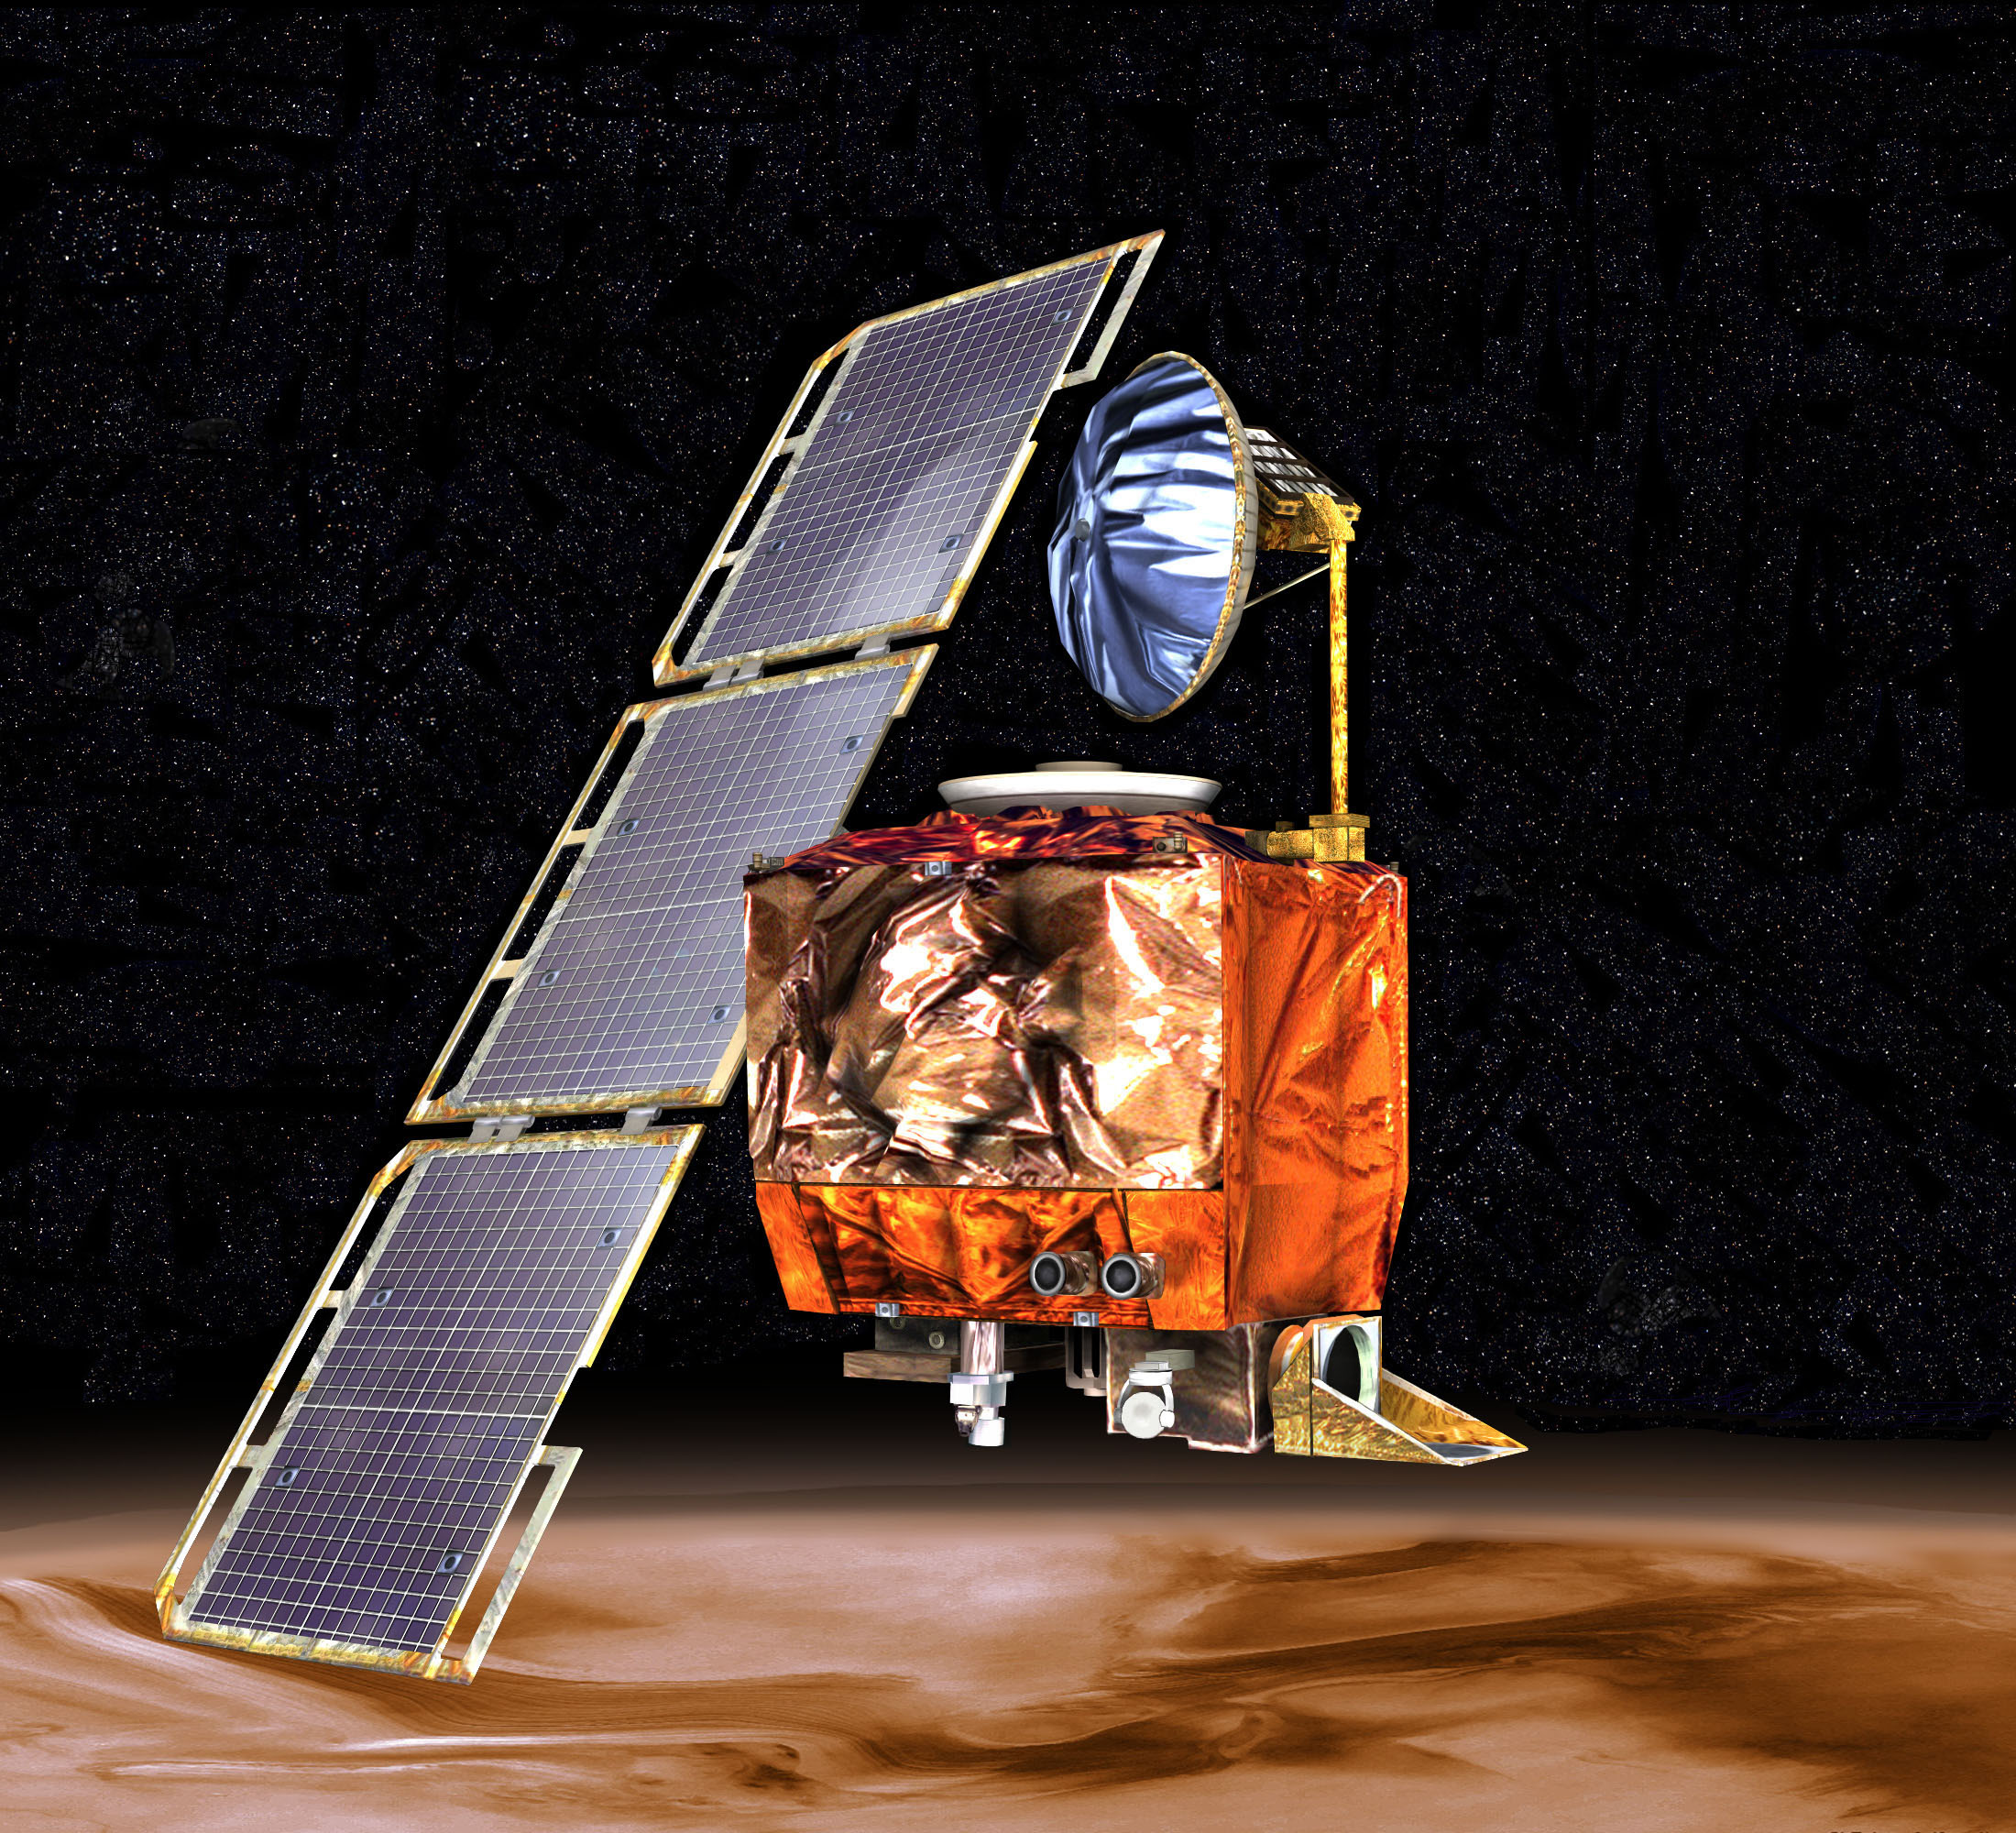
\includegraphics[width=0.9 \textwidth]{Mars_Climate_Orbiter_2.jpg}
  \end{minipage}
  \begin{minipage}{0.53 \textwidth}
    Mars Climate Orbiter (1998) \\[0.4cm]
    Cost of the mission: \\
    \$327 million \\[0.4cm]
    Failed due to a unit error \\
    {\small (newton-secs vs. pound-secs)}
  \end{minipage}

  \begin{center}
    \scalebox{3}{\Huge \frownie}
  \end{center}
\end{frame}

\begin{frame}[fragile]%\frametitle{Units of Measure}
  \begin{center}
    \vspace*{-1em}\Large\hil{Units of Measure Types \smiley}
  \end{center}
  \begin{minted}{text}
[<measure>] type N = (kg * m) / sec^2

fireThrusters (x:float<N * sec>) = ...

let duration = 2<sec>
let force = 1000<N>
fireThrusters (duration * force)

let diag (x:float<'u>) (y:float<'u>)
      = sqrt (x*x + y*y) // Pythagoras
  \end{minted}
\end{frame}

\begin{frame}%\frametitle{Units of Measure}
  \begin{center}
    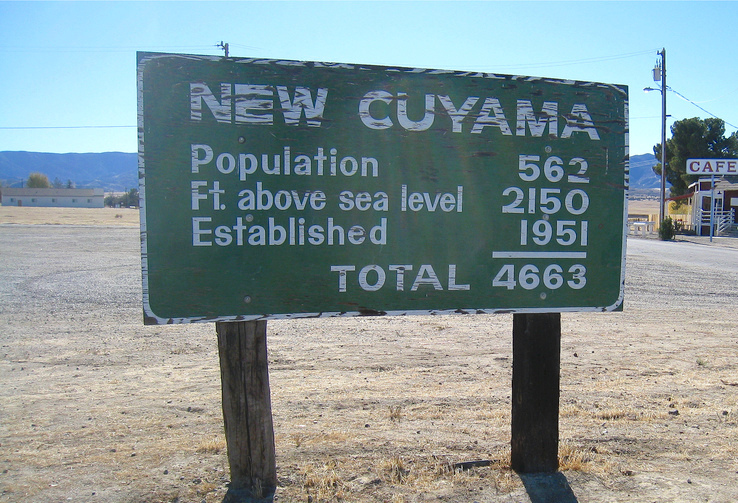
\includegraphics[width=11cm]{population_explosion.jpg}
  \end{center}
\end{frame}

\begin{frame}
  \begin{center}
    \vspace*{-1em}\Huge\hil{Time-traveling debugger}
    \medskip

    
\includegraphics[scale=0.7]{time-travel}
    % http://blogs.discovermagazine.com/crux/files/2014/01/time-travel-300x202.jpg
  \end{center}
\end{frame}

\begin{frame}
  \begin{center}
    \vspace*{-1em}\Huge\hil{Dependent types}
    \medskip
  \end{center}
\end{frame}
\end{document}

Brainstorm:

* "overloaded semicolon" to avoid callback hell (and mention monads) (Ingo)
* Maybe (Ingo)
* data structures & pattern matching (Ingo)
* Type system with type inference (Ingo)
* QuickCheck (Tim)
* time traveling debugger (Tim)
* Units of measure types (Tim)
* Regions from Rust


* STM


* DSLs
* meta programming
* Purity
* REPL with tab completion
* Regions von Rust?
* MonadFix?
* Listenmonade?
* Typklassen?
* List Fusion?
* LINQ
* Concurrency features
* probabilistic programming?
* dependent types?
